\documentclass[../Latex-Setup/setup.tex]{subfiles}
\graphicspath{{./images}}
\usepackage{listings}
\usepackage{xcolor}

\definecolor{codegreen}{rgb}{0,0.6,0}
\definecolor{codegray}{rgb}{0.5,0.5,0.5}
\definecolor{bgcolour}{rgb}{0.95,0.95,0.92}
\lstdefinestyle{code}{
    backgroundcolor=\color{bgcolour},   
    commentstyle=\color{codegreen},
    keywordstyle=\color{blue},
    numbers=none,
    %numberstyle=\tiny\color{codegray},
    basicstyle=\ttfamily\footnotesize,
    identifierstyle=\color{black},
    frame=L
}
\lstset{style=code}

\begin{document}
\title{Sets}
\author{Julian Dominic}
\date{\today}
\maketitle

\section{Introduction to Sets}

\indent A \textbf{set} is a collection of things. We call these things \textbf{elements}.
In Mathematics, we denote a set by writing elements inside curly brackets $\{a,b,c,d,\dots\}$.
For example, if we want a set to contain $2,4,6,8$ exactly, we can write it as $\{2,4,6,8\}$.
A set has either a \textbf{finite} or \textbf{infinite} amount of elements.
For example, we can have the set of all even integers:

\[\{\dots,-4,-2,0,2,4,\dots\}\]
the ellipsis (dots) here indicates that there are more elements, and since they are indicated at the `ends' of the sets,
we can say that numbers continues forever in both the negative and positive directions.\par

\indent Two sets are equal if they contain the \textbf{exact same elements regardless of their order}.

\[ \{1,2,3\} = \{3,1,2\} \]
\par

\indent We often let uppercase letters stand for sets. Lets say we have a set $A = \{2,4,6,8\}$, we can have some statements:

\begin{itemize}
    \item $2 \in A$: $2$ is an element of $A$; $2$ is in $A$; $2$ in $A$.
    \item $5 \notin A$: $5$ is not an element of $A$.
    \item $2,4,6,8 \in A$: $2,4,6,8$ are in $A$ -- this is how we can indicate that there are several things in a set.
\end{itemize}
\par

\indent \textbf{Cardinality} is how we can measure the size of the sets which is the number of elements in a set. 
For now, we will only concern ourselves where the sets are finite. If $X$ is a finite set, the cardinality of $X$ is $|X|$.\par

\indent There is a special set called the \textbf{empty set}, represented as $\emptyset$ or $\{\}$.
By its name, an empty set has no elements, thus, the cardinality $|\emptyset| = 0$. The empty set is the only set whose cardinality is zero.
We can think of a set as a ``box''. By this definition, the empty set is just an empty box. But what about $\{\emptyset\}$?
It is a box that contains an empty box, so we can say its cardinality $|\{\emptyset\}| = 1$.\par

\indent In Mathematics, we will often see/use the \textbf{set-builder notation} or some variant of it.
It is used to describe sets that are either too big, too complex or hard to list in standard $\{\}$ notation.

\[X = \{\text{expression}:\text{rule}\} \text{ or } \{\text{expression}|\text{rule}\}\]
this can be read as $X$ is the set of all things (elements) of the form ``expression'' such that ``rule''.
There can be many ways to express the same set. If we want to express the set of all even integers:
\begin{align*}
    E &= \{2n: n \in \ZZ\} \\
    &= \{n: n \text{ is an even integer}\} \\
    &= \{n: n=2k,k \in \ZZ\} \\
    &= \{n \in \mathbb{Z} : n \text{ is even}\}
\end{align*}
\par


\section{The Cartesian Product}

\indent The \textbf{Cartesian product} is an operation where we multiply two or more sets together to produce a new set.
To understand what the elements of this Cartesian product are, we need to know what is an ordered pair.
An \textbf{ordered pair} is a list $(x,y)$ of two things $x$ and $y$, enclosed in parentheses and separated by a comma.
As the name implies, while it may look similar to sets, an ordered pair cares about the order of its elements.
This is to show that we can have two ordered pairs -- $(2,4)$ and $(4,2)$ -- while they have the same elements,
they are not equal because the order of each element is different.\par

\indent The Cartesian product of two sets $A$ and $B$ can be written as $A \times B$. Note, the new set produced is called $A \times B$.
When there is a set, there will be its elements (unless it's the empty set):

\[A \times B =\{(a, b) : a \in A, b \in B\}\]
the elements of the Cartesian product of $A$ and $B$ are ordered pairs of the elements found in $A$ and $B$. For example,
$A = \{k, l, m\}$ and $B = \{q, r\}$, their Cartesian product $A \times B = \{(k,q), (k,r), (l,q), (l,r), (m,q), (m,r)\}$.
Do take note of the order of the elements within the ordered pairs, the elements of $A$ come first, followed by the elements of $B$.\par

\indent If $A$ and $B$ are finite sets, $|A \times B| = |A| \cdot |B|$.\par

\indent A quick note for programmers, if you haven't noticed it already, the Cartesian product is very similar to nested ``for'' loops!
\begin{lstlisting}[language=Python]
# Two Nested "For" Loops to illustrate the Cartesian Product
cartesian_product = []
A = [k,l,m]
B = [q,r]
for a in A:
    for b in B:
        ordered_pair = (a,b)
        cartesian_product.append(ordered_pair)

print(cartesian_product)  # [(k,q), (k,r), (l,q), (l,r), (m,q), (m,r)]
\end{lstlisting}
\par

\indent It is possible for one factor of a Cartesian product to be a Cartesian product too.
For example, $\RR \times (\NN \times \ZZ) = \{(x, (y,z)) : x \in \RR, (y,z) \in (\NN \times \ZZ)\}$.\par

\indent So far, we have been seeing Cartesian products between two sets, and we can also have Cartesian products with more than two sets.
Consider three sets, $\RR, \NN, \ZZ$. We will have a Cartesian product that has ordered triples.
$\RR \times \NN \times \ZZ = \{(x,y,z) : x \in \RR, y \in \NN, z \in \ZZ\}$.\par

\indent In general, with $n$-sets:

\[A_1 \times A_2 \times \dots \times A_n = \{(x_1,x_2,\dots,x_n) : x_i \in A_i \text{ for each } i = 1,2,\dots,n\}\]
Do take note of the placement of the parentheses when reading Cartesian products.
While $\RR \times \NN \times \ZZ$ and $\RR \times (\NN \times \ZZ)$ look the same, they really aren't the same.
The first Cartesian product is between three sets while the second Cartesian product is between two sets.\par

\indent For any set $A$ and positive integer $n$, the \textbf{Cartesian Power} $A^n$:

\[A^n = \underbrace{A \times A \times \dots \times A}_{n \text{ times}} = \{(x_1,x_2,\dots,x_n) : x_1,x_2,\dots,x_n \in A\}\]
\par

\indent The Cartesian power is more common than we think. The most common example so far is the case where $n = 1$ but we also see $n = 2$, and $n = 3$.
In particular, we can think of $\RR^2$ as the Cartesian plane that contains all the real numbers and $\ZZ^2$ as a grid of points on the Cartesian plane.
Physically, we can treat $\RR^2$ as a piece of paper, and $\ZZ^2$ are solid dots on the paper.
We can now draw links to coordinate geometry where we treat points in the forms of ordered pairs.
In this vein, we can say that $\RR^2$ is the combination of all possible coordinates on a real plane,
and $\ZZ^2$ is the combination of all coordinates whose elements are all integers.
For the case of $n = 3$, we can think of $\RR^3$ as the 3D space, and $\ZZ^3$ as a grid of points in the 3D space.\par

\indent Try sketching a few of the Cartesian powers such as $\ZZ^2, \ZZ^3, \NN^2, \NN^3$ to see it for yourself!\par

\begin{figure}[H]
    \begin{minipage}{0.45\textwidth}
    \centering
    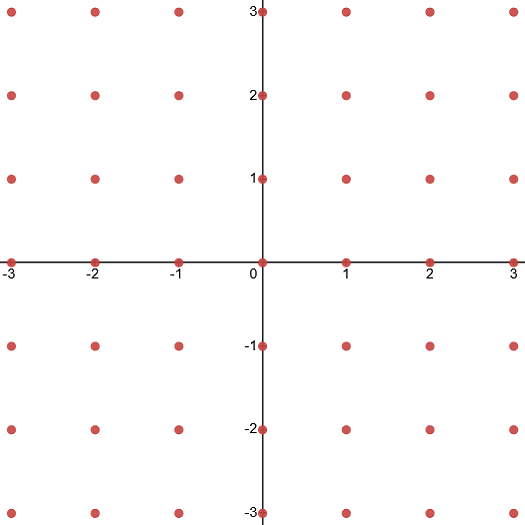
\includegraphics[scale=0.45]{./images/Z2-in-R2.png}
    \caption{$\ZZ^2$ in $\RR^2$ (Made in Desmos)}
    \end{minipage}\hfill
    \begin{minipage}{0.45\textwidth}
        \centering
        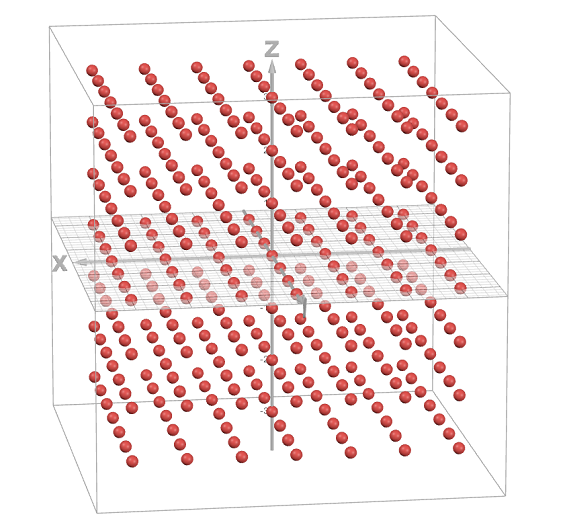
\includegraphics[scale=0.45]{./images/Z3-in-R3.png}
        \caption{$\ZZ^3$ in $\RR^3$ (Made in Desmos)}
    \end{minipage}
\end{figure}
\par

\begin{remark}
    Possible usage of intervals in Cartesian products.\par

    If you have any open or closed interval, you can treat the intervals as sets with an infinite number of elements.\par
    For example, suppose you have $[0, 1] \times [0, 1]$. Then the set produced will be something like:
    
    \[\{(0,0), (0,0.01), (0,0.001), \dots, (1,1)\}\]
    
    It would not be realistic to represent this in this set notation. Instead, we can represent visually with a graph.
    Earlier, we saw that we can treat each ordered pair as a collection of ``dots'' on the graph.
    When there are an infinite number of dots that are infinitesimally close to zero, they can be represented with a shaded region.
    In this case, it will be a shaded box of unit length with edges at $(0,0), (0,1), (1,0), (1,1)$.
\end{remark}

\section{Subsets}

\indent There can be cases where all the elements of a set $A$ is also the elements of another set $B$. For example,
every element in $A = \{a,b,c\}$ is also an element of $B = \{a,b,c,d\}$. When this case arises, we can say that $A$ is a \textbf{subset} of $B$.\par

\indent Suppose $A$ and $B$ are sets. If every element of $A$ is also an element of $B$, then we can say $A$ is a subset of $B$,
and it can be written as $A \subset B$. If $A$ is not a subset of $B$, it can be written as $A \not\subset B$ -- this means
that there is at least one element in $A$ that cannot be found in $B$.\par

\indent Here are some statements (\textit{most of them are important}) to take note of:
\begin{enumerate}
    \item $A \subseteq A$ for any set $A$
    \item $\emptyset \subseteq A$ for any set $A$
    \item $\emptyset \subseteq \emptyset$
    \item $\emptyset \notin \emptyset$
    \item $\NN \subset \ZZ \subset \QQ \subset \RR \subset \CC$
    \item $\RR \times \NN \subset \RR \times \RR$
    \item If a finite set has $n$ elements, then it has $2^n$ subsets (including $\emptyset$).
    \item $\NN \in \{\NN\}$
    \item $\NN \not\subset \{\NN\}$
\end{enumerate}
\par

\indent To see why (2) is true, think about the last sentence in the paragraph above. Consider the case where $\emptyset \not\subseteq B$ for any set $B$,
this will mean that there is at least one element in $\emptyset$ that is not in $B$. However, since $|\emptyset| = 0$, the statement that
``\textit{there is at least one element in $\emptyset$}'' is wrong, and fully invalidates the whole statement.
Hence, $\emptyset \not\subseteq B$ is false, so it must be the case that $\emptyset \subseteq B$.\par

\indent Moreover, another approach you can take is through the ``first principles''. When you construct a set, you start with an empty braces $\{\}$,
and you will fill up the braces with your elements or you can choose to leave it as an empty box. Thus, you are left with the subset $\{\}$,
which is mainly written as $\emptyset$; implying that $\emptyset \subseteq B$.\par

\indent It may be troubling to see why (9) is true. Go back to the definitions, lets take an element of $\NN$;
$1 \in \NN$, if $\NN \subset \{\NN\}$, this means that $1 \in \{\NN\}$. However, the only element in $\{\NN\}$ is $\NN$, $|\{\NN\}| = 1$.
Therefore, $\NN \not\subset \{\NN\}$.\par

\indent Another tricky example can be the following, suppose $B = \{a,b,\{c,d\}\}$. This means that $B$ has only $3$ elements, $a,b$, and $\{c,d\}$.
While $\{c,d\} \not\subset B$, it is true that $\{c,d\} \in B$. To make $\{c,d\}$ a subset of $B$, it has to be in a set itself -- $\{\{c,d\}\} \subset B$.\par

\begin{remark}
    Regarding the usage of $\subseteq$ and $\subset$. Suppose $A$ and $B$ are sets:\par
    \begin{itemize}
        \item $\subseteq$ is used when there's a possibility that the sets that are being compared, are equal -- $A = B$. This is called the ``improper subset.''
        \item $\subset$ is used when $|A| < |B|$ and $A \neq B$; all of $A$'s elements can be found in $B$ but the total number of elements is lesser than $B$. This is called the ``proper subset''.
    \end{itemize}
\end{remark}


\section{Power Sets}

\indent If $A$ is a set, the \textbf{Power Set} of $A$ is the set that contains all possible subsets of $A$, written as $\PP(A)$.
Using the set-builder notation, it can be written as $\PP(A) = \{X : X \subseteq A\}$.\par

\indent One common mistake to take note of is that since the power set is the set that contains all subsets, and subsets are still sets,
if you ever end up with an element in the power set that is not a set, be sure to double check your work!\par

\indent Following from the previous section, when we said if $|X| = n$, $X$ has $2^n$ subsets,
it implies that $|\PP(A)| = 2^{|A|}$.\par

\indent There is a way that I have developed on how to keep track of the subsets when writing out the power set:
\begin{enumerate}
    \item Write the empty set first, $\emptyset$
    \item Followed by each individual element contained in their own set, $\{a\}, \{b\}, \dots$
    \item Followed by the combination of sets that can be formed from each element put together
    \item Finally, write the set itself because $A \subseteq A$ for any set $A$
    \item It should look like $\PP(A) = \{\emptyset, \{a\}, \{b\}, \dots, A\}$.
\end{enumerate}
\par

\begin{example}
    Here are some examples to think about:
    \begin{itemize}
        \item $\PP(\emptyset)=\{\emptyset\}$
        \item $\PP(\{a\})=\{\emptyset, \{a\}\}$
        \item $\PP(\{\emptyset\}) = \{\emptyset, \{\emptyset\}\}$
        \item $\PP(\PP(\{\emptyset\}))=\{\emptyset, \{\emptyset\}, \{\{\emptyset\}\}, \{\emptyset, \{\emptyset\}\}\}$
        \item $\PP(\{a\}) \times \PP(\{\emptyset\}) = \{(\emptyset, \emptyset), (\emptyset, \{\emptyset\}), (\{a\}, \emptyset), (\{a\}, \{\emptyset\})\}$
    \end{itemize}
\end{example}


\section{Union, Intersection, Difference}

\indent Suppose $A$ and $B$ are sets. The \textbf{union} of $A$ and $B$ is the set of all things that are in $A$ or in $B$ or in both.
Take note that this is an inclusive ``or''. It can be written as $A \cup B$ which represents $\{x : x \in A \text{ or } x \in B\}$.\par

\[A \cup B = B \cup A\]
\par

\indent The \textbf{intersection} of $A$ and $B$ is the set of all things that are in both $A$ and $B$.
It can be written as $A \cap B$ which represents $\{x : x \in A \text{ and } x \in B\}$.\par

\[A \cap B = B \cap A\]
\par

\indent The \textbf{difference} of $A$ and $B$ is the set of all things that in $A$ but not in $B$.
It can be written as $A - B$ which represents $\{x : x \in A \text{ and } x \notin B\}$.\par

\[A - B \neq B - A\]
\par

\begin{example}
    \indent Here are some examples for you to gain a better understanding of the operations.
    Suppose $A = \{a,b,c\}$, $B = \{b,c,d\}$, and $C = \{0,1\}$\par
    \begin{itemize}
        \item $A \cup B = \{a,b,c,d\}$. Since a set only has unique elements (\textit{elements that appear at most once}), the elements cannot be repeated!
        \item $A \cap B = \{b,c\}$
        \item $A - B = \{a\}$
        \item $A \cap C = \emptyset$
    \end{itemize}
\end{example}


\section{Complement}
\section{Venn Diagrams}
\section{Indexed Sets}
\section{Sets That Are Number Systems}
\section{Russell's Paradox}
\end{document}